\documentclass[sigconf]{acmart}
\usepackage{booktabs} % For formal tables
\usepackage{comment}
\newcommand\tab[1][0.5cm]{\hspace*{#1}}
\usepackage{float}

% Copyright
%\setcopyright{none}
%\setcopyright{acmcopyright}
%\setcopyright{acmlicensed}
% \setcopyright{rightsretained}
%\setcopyright{usgov}
%\setcopyright{usgovmixed}
%\setcopyright{cagov}
%\setcopyright{cagovmixed}


% DOI
% \acmDOI{10.475/123_4}

% ISBN
% \acmISBN{123-4567-24-567/08/06}

%Conference
\acmConference[CIKM'17]{International Conference on Information and Knowledge Management}{6-10 Nov. 2017}{Pan Pacific Singapore} 
\acmYear{2017}
\copyrightyear{2017}

% \acmPrice{15.00}


\begin{document}
%\title{Lazada Product Title Quality Challenge: 2nd Place Approach}
\title{Bagging Model for Product Title Quality with Noise}
\titlenote{The source code is available at https://goo.gl/1dmsXZ}
\subtitle{CIKM AnalytiCup 2017}
\subtitlenote{https://competitions.codalab.org/competitions/16652}

\author{Tam T. Nguyen}
\authornote{Laboratory for Systems, Software and Semantics, Ryerson University}
% \orcid{}
\affiliation{
\institution{Ryerson University}
% \streetaddress{}\city{Toronto}\state{ON.}\postcode{}\country{Canada}
}
\email{nthanhtam@gmail.com}

\author{Hossein Fani}
\authornotemark[3]
\orcid{0000-0002-6033-6564}
\affiliation{\institution{University of New Brunswick}
% \streetaddress{}\city{Fredericton}\state{NB.}\postcode{}\country{Canada}
}
\email{hosseinfani@gmail.com}

\author{Ebrahim Bagheri}
\authornotemark[3]
\affiliation{\institution{Ryerson University}
% \streetaddress{}\city{Toronto}\state{ON.}\country{Canada}
}
\email{ebrahim.bagheri@gmail.com}

\author{Gilberto Titericz}
\affiliation{\institution{Airbnb, Inc.}
% \city{Sans Francisco}\state{CA}\country{USA}
}
\email{giba1978@gmail.com}

% The default list of authors is too long for headers}
\renewcommand{\shortauthors}{T. Nguyen et al.}


\begin{abstract}
We present our winning approach for the Lazada Product Title Quality Challenge for the CIKM Cup 2017 where the data set was annotated as \textit{conciseness} and \textit{clarity} by Lazada QA staffs. The participants were asked to build machine learning model to predict \textit{conciseness} and \textit{clarity} of an SKU based on product title, short description, product categories, price, country, and product type. As sellers could freely enter anything for title and description, they might contain typos or misspelling words. Moreover, there were many annotators labelling the data so there must be disagreement on the true label of an SKU. This makes the problem difficult to solve if one is solely using traditional natural language processing and machine learning techniques. In our proposed approach, we adapted text mining and machine learning methods which take into account both feature and label noises. Specifically, we are using bagging methods to deal with label noise where the whole training data cannot be used to build our models. Moreover, we think that for each SKU, \textit{conciseness} and \textit{clarity} would be annotated by the same QA. It means that \textit{conciseness} and \textit{clarity} should be co-related in a certain manner. Therefore, we extended our bagging approach by considering out of fold leakage to take advantage of co-relation information. Our proposed approach achieved the root mean squared error (RMSE) of 0.3294 and 0.2417 on the test data for \textit{conciseness} and \textit{clarity}, respectively. 

\end{abstract}

%
% The code below should be generated by the tool at
% http://dl.acm.org/ccs.cfm
% Please copy and paste the code instead of the example below. 
%

\keywords{Product Title Quality, E-Commerce, CIKM AnalytiCup}


\maketitle

\section{Introduction}
Customers do indeed fall prey to cognitive bias of `judging a book by its cover' and product's title functions as the sole factor influencing their decision of whether to buy or skip a particular product. As a result, titling of a product becomes essential in e-commerce for sellers. Sellers attempt a clear, yet concise title which not only describes a product and its features comprehensively, but also stands out the product among all the likes in the result of product search engines for customers. However, seeking customer's attention, some inexperienced or malicious sellers might choose inaccurate or fraudulent titles such as \textit{`Hot Sexy Tom Clovers Womens Mens Classy Look Cool Simple Style Casual Canvas Crossbody Messenger Bag Handbag Fashion Bag Tote Handbag Gray'}. 

In the Lazada product title quality challenge, given a set of product titles, description, and attributes, we aim to build a product title quality model that can assess the \textit{clarity} and the \textit{conciseness} of a product title systematically and automatically, concluding to a state of clean and relevant product titles. Specifically, we have defined two independent neural-based regressors to rate the quality measures, clarity and conciseness, based on the feature set including n-gram character of the product title and other features such as title length, description length, number count. 

%We evaluate our final proposed model by using the root mean square error (RMSE) for clarity and conciseness separately. Our model ranks 2nd in clarity and 3rd places in conciseness respectively ahead of more than 150 participants. The average of the clarity and the conciseness's RMSE ranks our model to the 2nd place overall. 

\begin{comment}
\section{Related Work}
Product title has been of interest from product categorization point of view as in \cite{DBLP:conf/eacl/ShinzatoDXLFD17, DBLP:journals/ijon/ShenRMS12, DBLP:conf/kdd/HaPK16, DBLP:conf/cikm/ShenRS12}. Such works and the likes in this area have been already points out the noise issues that arise in large product datasets and tried to build robust classifiers. However, to the best of our knowledge, Lazada product title quality challenge is the first who attempts to address the noise in product title particularly. 

\section{Problem Definition}
Given a product $p\in\mathcal{P}$, we aim at learning \textit{clarity} and \textit{conciseness} of the $p$'s title through two boolean target functions $f$ and $g$ which maps $\mathcal{P}$ to $\{0, 1\}$, indicating whether $p$'s title is clear, concise, or both. 

\end{comment}

\section{Dataset}
We evaluate our proposed model on a data set of more than 60K products from Lazada, southeast Asia's number one online shopping and selling destination.  Besides its title, each product is accompanied by id, three-level hierarchical category, description, price, country of origin, delivery scope. % as shown in Table~\ref{tbl:dataset}.

\begin{comment}
\begin{table*}
\small
    \caption{Lazada Dataset Description.}
    \label{tbl:dataset}
    \begin{tabular}{lll} \hline
      \textbf{name} & \textbf{description} & \textbf{example}  \\ \hline 
      sku\_id & unique product id & \textit{NO037FAAA8CLZ2ANMY}  \\ %\hline
      title & product title & \textit{RUDY Dress}  \\ %\hline 
      country & the country where the product is marketed & \textit{my} for Malaysia, \textit{ph} for Philippines, \textit{sg} for Singapore  \\  %\hline
      category\_lvl\_1 & general category & \textit{Fashion}  \\ %\hline 
      category\_lvl\_2 & intermediate category & \textit{Women} \\  %\hline 
      category\_lvl\_3 & specific category & \textit{Clothing}   \\ %\hline
      short\_description & short description of the product & \textit{<ul> <li>Short Sleeve</li> <li>3 Colours 8 Sizes</li> <li>Dress</li> </ul> } \\ %\hline 
      price & price in the local currency & \textit{33.0}. if `country' is \textit{my}, the price is in Malaysian Ringgit.  \\&&\hspace{22mm}\textit{sg}, the price is in Singapore Dollar.  \\&&\hspace{22mm}\textit{ph}, the price is in Philippine Peso.  \\ %\hline 
      product\_type & product type & \textit{local} means the product is delivered locally,\\&& \textit{international} means the product is delivered from abroad, \\&&\textit{NA} means not applicable. \\ \hline 
    \end{tabular} 
\end{table*}

\end{comment}
\begin{table*}[t]
\small
\centering
\caption{Disagreement in target functions clarity and conciseness for similar titles.}
\label{tbl:noise}
\begin{tabular}{ll|cc}
\hline
\textbf{sku\_id} & \textbf{title}                                                                & \textbf{clarity} & \textbf{conciseness} \\ \hline
%\textit{NO037ELAA53HC0ANMY}          & \textit{JOR Computer USB Flash Drive 16GB Memory Stick Pendrive (Black/Silver)}                    & 0       & 1           \\
%\textit{NO780ELAA4BAOTSGAMZ}         & \textit{JOR Computer USB Flash Drive 64GB Memory Stick Pendrive (Black Silver)(Export)}            & 1       & 1           \\ \hline
\textit{VO749FAAAAD86YANMY}          & \textit{1 Pair of Unisex Touch Screen Sensitive Gloves Knitted Winter Warm Christmas Glove Coffee} & 0       & 1           \\
\textit{VO749FAAAAD7E8ANMY}          & \textit{1 Pair of Unisex Touch Screen Sensitive Gloves Knitted Winter Warm Christmas Glove Red}    & 0       & 0          \\ \hline
\end{tabular}
\end{table*}
\begin{figure}[t]
\centering
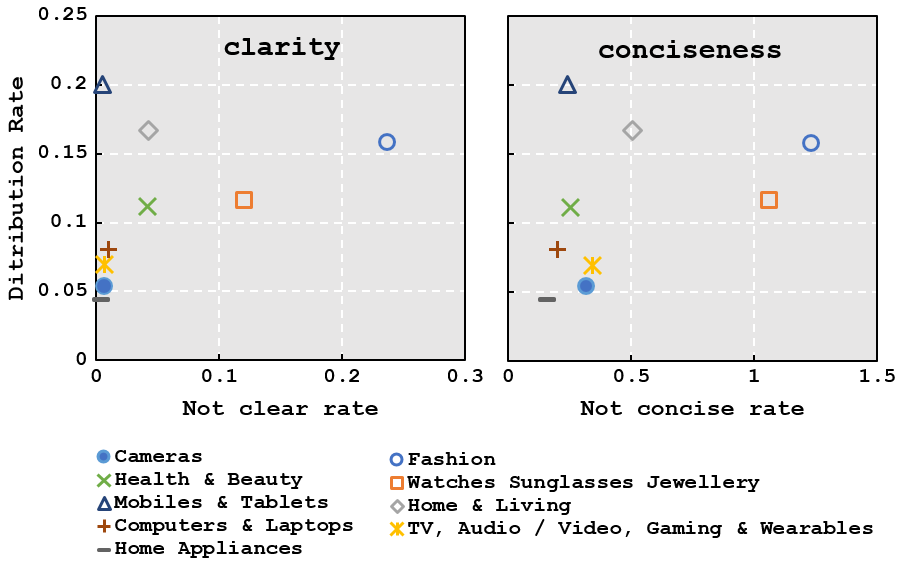
\includegraphics[width=0.45\textwidth]{dist_not_clarity_not_concise.png}
\caption{Distribution of product general categories (category\_lvl\_1) vs. not clear and not concise target functions.\label{fig:dist_not_clarity_not_concise}}
\end{figure}
Additionally, the product title's clarity and conciseness are measured manually by Lazada's internal quality control team based on the following guidelines:

\begin{itemize}
    \item \textbf{clarity:} The product title is clear if within five seconds one can understand the title, what the product is, and quickly figure out the key attributes (color, size, model, ...). 
    %Otherwise, i.e., one is not sure what the product is after five seconds and have to read the title more than once, the product title is not clear.
    \item \textbf{conciseness:} The product title is concise if it is short enough to contain all the necessary information. Otherwise, i.e., the title is too long with many unnecessary words, Or it is too short such that it is unsure what the product is.

\end{itemize}

\subsection{Data Exploration}
We first explore the data at each product instance including clarity and conciseness labels. We found that the dataset has outliers in `price' (-1, 999999, 9999999). More importantly, we discover that there are some disagreement in titles' clarity and conciseness such that very similar titles receive different judgments as in Table~\ref{tbl:noise}. %We conclude that the target functions do not only depend on the product title and other properties have influence. 

Secondly, we inspect each property to find more pieces of information. We found that the first 2 characters in `sku\_id' and product brand name are often but not always the same. Brand names also happen to be the first term of `title'. %Also, `short\_description' include html image tag (<img>) with a link to an product image. As a result, brand name and image could potentially be added as extra features.

\begin{comment}
\begin{table*}[]
\small
\centering
\caption{Brand name extraction.}
\label{tbl:brandname}
\begin{tabular}{ll|cc}
\hline
\textbf{sku\_id} & \textbf{title}                                                                                            & \textbf{brand}   \\ \hline
\textit{\textbf{AR}511HBAXNWAANMY}   & \textit{\textbf{Argital} Argiltubo Green Clay For Face and Body 250ml}                                               & ARGITAL \\
\textit{\textbf{AS}575ELCMZ4WANMY}   & \textit{\textbf{Asus} TP300LJ-DW004H Transformer Book Flip 4GB Intel Core i5 13 Inch + Free 2Year Ezi Care Warranty} & ASUS    \\
\textit{\textbf{EL}802HLAA51ZZVANMY} & \textit{\textbf{ELENXS} Stainless Steel Tea Ball Strainer Mesh Infuser Filter  Sphere  7Cm} & ELENXS  \\ \hline
\end{tabular}
\end{table*}

\end{comment}

Thirdly, we also check the correlation of the two labels. Interestingly, we found that there are only three combinations for the pair. While titles which are clear might be concise or not, there are no title which is not clear, yet concise. Intuitively, if a title is not clear, it is not concise either. 

%In another word and by contraposition, we have if a title is concise then it is clear as well; ${\sim}f(p)\to{{\sim}g(p)}$ and $g(p)\to{f(p)}$. This finding could provide us to employ multi-output classification approaches where a single model(estimator) is learned to predict both target functions instead of two independent ones. We have tried variants of such approaches. While multi-output models require lower training time since only a single estimator is built, the generalization accuracy was not improved significantly with compare to our final solution which include two separate neural-based regressor for each target functions of clarity and conciseness.

Finally, we study the distribution of products over clarity and conciseness based on different categories as shown in Figure~\ref{fig:dist_not_clarity_not_concise}. Compared to other categories, Fashion and Watches categories is quite balanced that makes prediction problem easier on these categories.

\begin{comment}
\section{Evaluation Metric}
The goal of the competition is to estimate the quality of product title with respect to two target functions: clarity and conciseness. The evaluation metric is the root mean square error (RMSE), defined as follows:

\begin{equation}\label{eq:rmse}
    RMSE_y = \sqrt{\frac{\sum_{p\in\mathcal{P}}{(\hat{y}(p)-y(p))^2}}{|\mathcal{P}|}}
\end{equation}
where $\mathcal{P}$ is the number of products,  $\hat{y}(p)\in\mathcal{R}^{[0,1]}$ is the predicted probability value for a given product $p$, and  $y\in\{0,1\}$ is the ground-truth value. The RMSE is calculated separately for clarity $f$ and conciseness $g$ and the overall leaderboard ranking is based on the the average. i.e.,
\begin{equation}\label{eq:overal_rmse}
    \overline{RMSE} = \frac{RMSE_f + RMSE_g}{2}
\end{equation}
The lower the average, the higher is the ranking.

\end{comment}

\section{Proposed Approach}
In this section we describe our proposed approach including feature engineering and modelling.
\begin{comment}
\subsection{Preprocessing}
We did cleansing by removing the html tags in `short\_description' values. Also, we normalize `price' values based on the `country' to a single currency. No imputation has been done for missing values in `category\_lvl\_3' and `short\_description' attributes.
\end{comment}

\subsection{Feature Engineering}
Before extracting features, we preprocess the data by removing HTML tags, removing special characters, and replacing missing values.
\subsubsection{Feature Extraction}
Besides the non-textual attributes of the products such as `price' or category information, we focus on extracting more information from the textual attributes, `title' and `short\_description'. Our features fall into the 9 groups as explained in Table \ref{tbl:features}.
\begin{table}[]
\small
\centering
\caption{All features set.}
\label{tbl:features}
\begin{tabular}{lll}
\hline
\textbf{group} & \textbf{features} & \textbf{name} \\ \hline
statistics&\#char(length)\\&\#term & xg\_feat \\& price & price\_feat \\ %\hline
information&color & color\\&brand&brand\\&category entropy & entropy\_feat\\ %\hline
n-gram term& (1,3)-gram & bow.3grams \\
n-gram char&(1,6)-gram & boc.6grams\\&\#upper char\\&\#special char\\&html escape\\&\#invisible char\\ %\hline
sparse feature &  category one-hot-encoding & sp\_feat\\
leave-one-out encode & \\
embedding&word2vec\cite{DBLP:conf/nips/MikolovSCCD13}\\
%&GloVe\cite{DBLP:conf/emnlp/PenningtonSM14}'s pre-trained word vectors\\ %\hline
part-of-speech&\#adjective\\&\#verb\\&\#noun\\&\#number\\ %\hline
multilingual characters&\#non-english char\\&\#chinese char & char\_set\_feat \\ %\hline
%reading ease&\#syllable\\&average \#letter in word\\& average \#syllable in word\\&Coleman-Liau index\cite{}\\& Dale-Chall readability score\cite{}\\& automated readability index\cite{}\\& \#difficult word\\& Flesch reading ease\cite{}\\& Flesch-Kincaid grade\cite{}\\& Gunning-Fog\cite{}\\& Smog index\cite{}\\

\hline
\end{tabular}
\end{table}

\begin{comment}
\subsubsection{Feature Reduction}
We employed latent semantic analysis (LSA)\cite{}, principal component analysis (PCA)\cite{}, linear singular value decomposition \cite{}(SVD), and t-distributed stochastic neighbor embedding (t-SNE) \cite{} of n-gram term as well as n-gram character features of `title' and `short\_descrition' to project them to a lower dense dimensional space. 

\end{comment}
\begin{table}[]
\small
\centering
\caption{Most important features based on linear SVM.}
\label{tbl:top_features}
\begin{tabular}{lll|lll}
\hline
\textbf{label} &\textbf{name} & \textbf{coef.} & \textbf{label} &\textbf{name} & \textbf{coef.} \\ \hline
clarity
&t     &0.442989 & conciseness & my     &   1.087967\\
&sexy  &   0.398171 & & ph     &   0.968527\\
&exy   &  0.398026 & & c      &  0.957356\\
&sex   &  0.384535 & & ocal   &     0.931618\\
&urse  &   0.368735 & & local  &      0.925727\\
&purse &    0.341463 & & r      &  0.920576\\
&purs  &   0.341463 & & loca   &     0.912073\\
&rse   &  0.338007 & & sg     &   0.909163\\
&xy    & 0.334105 & & cal    &    0.888805\\
&purse &    0.326108 & & loc    &    0.882074\\
%&urs   &  0.320952\\
%&sb    & 0.316896\\
%&tc    & 0.314088\\
%&purs  &   0.312165\\
%&sbe   &  0.302878\\ \hline

%& t      &  0.858808\\
%& ch     &   0.853172\\
%& oca    &    0.850233\\
%& my     &   0.820174\\
%& se     &   0.815047\\
%& e      &  0.811894\\
%& bag    &    0.799149\\
\hline
\end{tabular}
\end{table}

\begin{figure*}
  \centering
    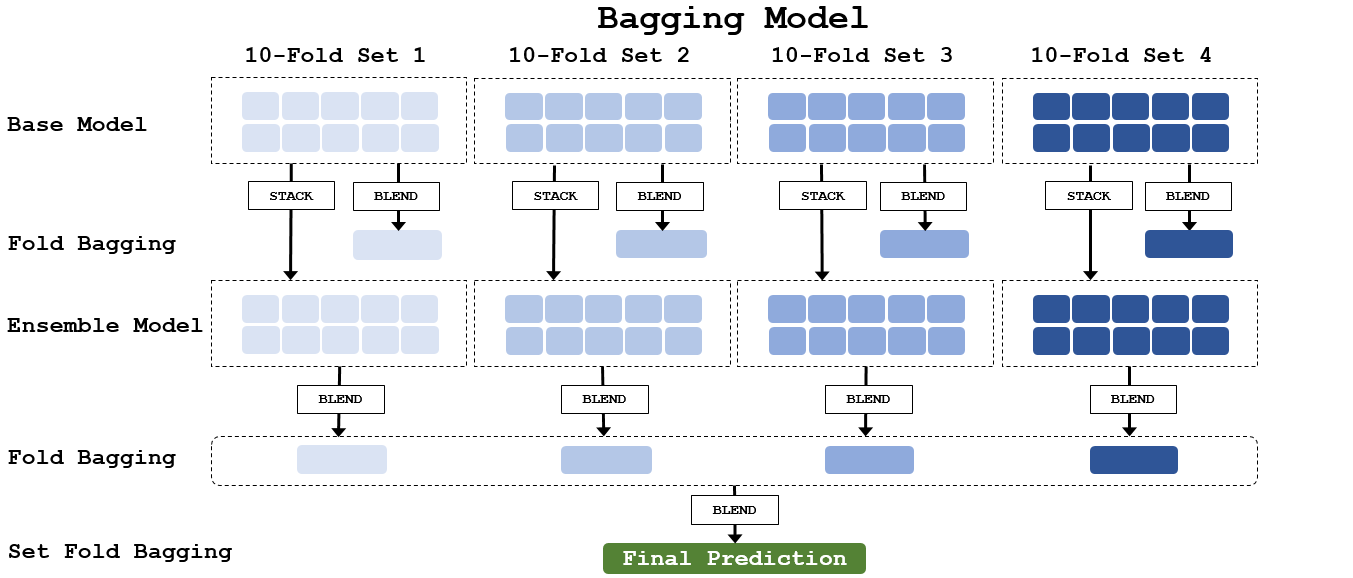
\includegraphics[width=\textwidth]{cikm_cup_model_new}
  \caption{Product title quality modelling.}
  \label{fig:model}
\end{figure*}
\subsubsection{Feature Selection}
%In order to select features which have the most contribution to the quality target functions, clarity $f$ and conciseness $g$, among about *** features, we have removed those whose variance is small as a sign that almost values are the same and, thus, there could be no contribution. Then, we used statistical tests, namely $\chi^2$ and f-test, to find linear correlation and mutual information \cite{} to find any type of correlation between each feature and target functions. 

For feature selection, based on estimators such as linear or tree-based models, one can identify the most importance features as well. For instance, linear models which penalized with the $\mathcal{
\ell}_1$-norm have sparse solutions and most of their estimated coefficients are zero. Non-zero coefficient of a feature, therefore, shows its importance. In our work, we use linear SVM to identify our best features as listed in Table~\ref{tbl:top_features}. We can see that 'sexy' and 'purse' are among the important features of clarity models, namely top\_clarity. These features often come from Fashion category. On the other hand, 'my' and 'ph' are important features of conciseness models, namely top\_conciseness. These feature represent the location where the products are being sold. We use these top features to train our predictive models which will be presented in the next section.

\begin{comment}
\subsubsection{Data Augmentation}
We increase the size of our training set by systematic data augmentation. Data augmentation prevent overfitting which helps our model to be more robust and simpler. To this end, we replicate a product through permutation on its color and brand as these attributes do not have contribution to the target functions intuitively. Therefore, we create different copy of a product by replacing color and brand names in its title while preserving same target function values. 

\end{comment}

\subsection{Product Title Quality Modelling}
As shown in Table~\ref{tbl:noise}, there is disagreement in the training labels where the same titles have different labels. Therefore, if we use the whole training data set, these noises make machine learning model work worse. However, if one uses less training data, one may loose some important information. This leads to building less accurate models. To overcome the issue, we propose a bagging method which not only leverages all training data but also reduces noises in the training data. The proposed approach is shown in Figure~\ref{fig:model} which consists of fold set generation, base model training, ensemble model building, and blending.

\subsubsection{Fold Set Generation}
To reduce label noise in the training data, we manage to use subsets of training data to build our models. In order to do that, we use 10-fold cross validation process to split the data into 10 separate folds. As the data is randomly partitioned, we don't know which one is the best split. Therefore, we apply the k-fold process 4 times to get 4 different fold sets. We then use 9 folds to train our machine learning models and make predictions for the testing data. So for each fold set, we have 10 models and 10 testing predictions, we finally blend 10 predictions to have the final predictions. 

\subsubsection{Base Model}

We use stratified 10-fold cross validation process to evaluate the performance of our models. We train different estimators such as extreme trees (ETC), random forest (RFC), stochastic gradient descent (SGD), logistic regression (LOR), ridge regression (RDG), naive bayes (NBC) using Scikit-Learn~\cite{scikit-learn}; extreme gradient boosting (XGB)~\cite{DBLP:conf/kdd/ChenG16}; light gradient boosting (LGB); and word2vec (W2V). 

The performance results are shown in Figure~\ref{fig:con_base_model_rmse} and Figure~\ref{fig:cla_base_model_rmse} for conciseness and clarity labels, respectively. In both labels, LGB has the RMSE of $0.3198$ which outperforms other algorithms, XGB is the runner up and the next one is Logistic Regression. Finally, the worst model is Naive Bayes algorithm whose RMSE is $0.4047$. 

Similarly, LGB is also the best algorithm for predicting clarity label. While clarity RMSE of LGB is $0.2098$, that of XGB is $0.2102$. Notably, W2V model works quite well on clarity label. Its performance is just after logistic regression (LOR) and it also contribute to the performance of ensemble model that will be discuss in the next section. Although other algorithms such as naive bayes (NBC) and stochastic gradient descent (SGD) do not work well in this data, they can help improve the performance of ensemble models. Therefore, we keep these models in our final solution.

For each algorithm, we build 10 models and make 10 testing predictions. The final testing output is generated by blending these 10 predictions. We repeat these process on 4 fold sets as mentioned in the previous section.
\begin{figure}
  \centering
    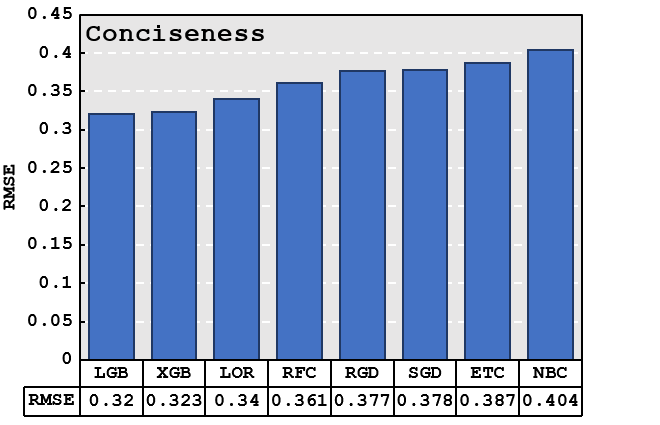
\includegraphics[width=0.38\textwidth]{conciseness_base_model_rmse_new}
  \caption{Base model performance for conciseness.}
  \label{fig:con_base_model_rmse}
\end{figure}

\subsubsection{Stacked Ensemble Model}
In order to combine base models together, we apply stacked ensemble method. It means that we used validation predictions to train another models and make testing predictions using testing predictions of base models. We have tried a few algorithms for stacking but we found that XGB is the best. Therefore, we only use XGB for our ensemble models. The performance of ensemble models are shown in Table~\ref{tbl:ensemble_model_rmse} where RMSEs of XGB for both conciseness and clarity are $0.31553$ and $0.20745$ respectively. Comparing to the best base model, the improvement is $0.004$ for conciseness and $0.002$ for clarity.

\subsubsection{Model Selection}
We also study the importance of base model in ensemble models. The results are shown in Table~\ref{tbl:base_conciseness} and Table~\ref{tbl:base_clarity}. Interestingly, while the most important models for conciseness are LGB models, those for clarity are SGD and W2V models. It means that clarity label is sensitive to noise so linear models can help reduce it significantly. Moreover, RDG trained on clarity label is also a good contributor of ensemble conciseness models.

\subsubsection{Final Solution}
Our final solution is the blended predictions of 4 fold sets. After training ensemble model and making predictions for each fold sets. We first combine 10 models for each fold set to have 4 testing predictions. We then blend the predictions by averaging them to have the final prediction. 

\section{Lessons Learned}
We have tried many NLP techniques such as stemming, stop-words removal, POS tagging, topic extracting but none of them worked. The key feature set for this problem is character ngrams. We found that term frequency works better than other unsupervised and supervised term weighting techniques~\cite{nguyen11}. Moreover, we tried dimension reduction technique such as latent semantic analysis (LSA) and principle component analysis (PCA) but they did not work. We also used recent deep learning techniques like attention model and we failed to have a useful model. Maybe short description is irrelevant to this problem or the QA staffs have not considered it when labelling the data.

\section{Conclusion}
In this paper, we have presented our winning solution for product title quality analysis. The proposed approach which uses powerful machine learning algorithms such as light gradient boosting (LGB), extreme gradient boosting (XGB) with traditional features in text mining such as word n-grams and character n-grams gives state-of-the-arts performance. We hope that our solution will probably provide a benchmark for solving product title quality analysis as well as other text classification problems in e-commerce.
\begin{figure}
  \centering
    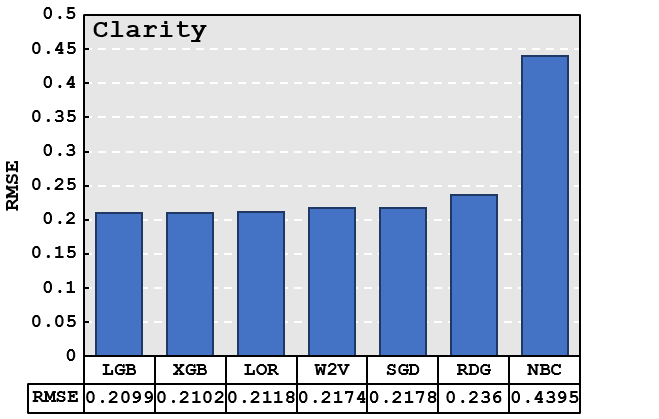
\includegraphics[width=0.38\textwidth]{clarity_base_model_rmse_new}
  \caption{Base model performance for clarity.}
  \label{fig:cla_base_model_rmse}
\end{figure}
\begin{table}[]
\small
\centering
\caption{Ensemble model performance.}
\label{tbl:ensemble_model_rmse}
\begin{tabular}{l l l}
\hline
\textbf{label} & \textbf{algorithm} & \textbf{RMSE} \\ \hline
conciseness & XGB & 0.31553 \\
clarity & XGB & 0.20745 \\

\hline
\end{tabular}
\end{table}

\begin{table}[t]
\small
\centering
\caption{Top base models for conciseness.}
\label{tbl:base_conciseness}
\begin{tabular}{l p{3.5cm} l}
\hline
\textbf{algorithm} & \textbf{feature set} & \textbf{importance} \\ \hline

SGD & title.boc.6grams &	0.017230835 \\
%SGD & title.boc.6grams sp\_feat title.color title.brand &	0.016379929 \\
W2V & glove.twitter.27B.200d & 0.015874704 \\
NBC & title.boc.5grams &	0.015768725 \\
LOR & title.boc.6grams & 0.014890845 \\
%W2V & glove.twitter.27B.100d & 0.013960167 \\
LGB & title.boc.6grams, xg\_feat title.color, title.brand, title.glove.twitter.27B.25d\_mean price\_feat, entropy\_feat, top\_clarity, char\_set\_feat & 0.013428351 \\
%W2V & glove.6B.200d & 0.01273699 \\
%XGB & title.boc.6grams xg\_feat title.color title.brand item\_cnt cat\_cnt\_feat title\_cat\_feat & 0.012657218 \\

\hline
\end{tabular}
\end{table}

\begin{table}[t]
\small
\centering
\caption{Top base models for clarity.}
\label{tbl:base_clarity}
\begin{tabular}{l p{3.5cm} l}
\hline
\textbf{algorithm} & \textbf{feature set} & \textbf{importance} \\ \hline

LGB & title.boc.6grams, xg\_feat title.color, title.brand, item\_cnt, cat\_cnt\_feat, title\_cat\_feat &	0.02956636 \\
%LGB & title.boc.6grams xg\_feat title.color title.brand title.glove.twitter.27B.25d\_mean price\_feat & 0.022996058 \\
%LGB & title.boc.6grams xg\_feat title.color title.brand &	0.021024967 \\
XGB & giba\_clar &	0.020367937 \\
%LGB & title.boc.6grams xg\_feat title.color title.brand title.glove.twitter.27B.25d\_mean &	0.015768725 \\
%LGB & title.boc.6grams xg\_feat title.color title.brand title.glove.twitter.27B.25d\_mean title.glove.6B.50d\_mean &	0.015111695 \\
RDG & title.boc.6grams, sp\_feat, title.color, title.brand & 0.015111695 \\
XGB & title.boc.6grams xg\_feat title.color title.brand item\_cnt cat\_cnt\_feat title\_cat\_feat &	0.013797635 \\
%RDG & title.boc.6grams &	0.013428351 \\
%LGB & title.boc.6grams xg\_feat title.color title.brand item\_cnt &	0.013797635 \\
SGD & title.boc.5grams, sp\_feat &	0.011826544 \\
\hline
\end{tabular}
\end{table}

\bibliographystyle{ACM-Reference-Format}
\bibliography{bibliography} 

\end{document}
